\documentclass[../hewa_main-subfiles.tex]{subfiles}
\graphicspath{{\subfix{../../Images/}}}

\begin{document}

\section{Introduction}

%General info about the language
%Previous documentation: Klamer wordlist

Hewa is a language variety spoken in the village of the same name, in the eastern part of the island of Flores in eastern Indonesia.\footnote{The Hewa language of Flores is not to be confused with a language of the same name spoken in Papua New Guinea, ISO 639-3: ham.} Hewa is also known as Sika Krowe by speakers of neighboring varieties. It is considered a dialect of the better documented Sika language (ISO 639-3: ski), spoken along eastern Flores (see \cref{fig:langmap}), and which belongs to the Central-Eastern Malayo-Polynesian group in the Austronesian family \citep{Lewis1995}. Sika is estimated to have approximately 175,000 speakers \citep{Lewis1995}.

%TODO Maybe include typological info on the language(extra)

\begin{figure}[h]

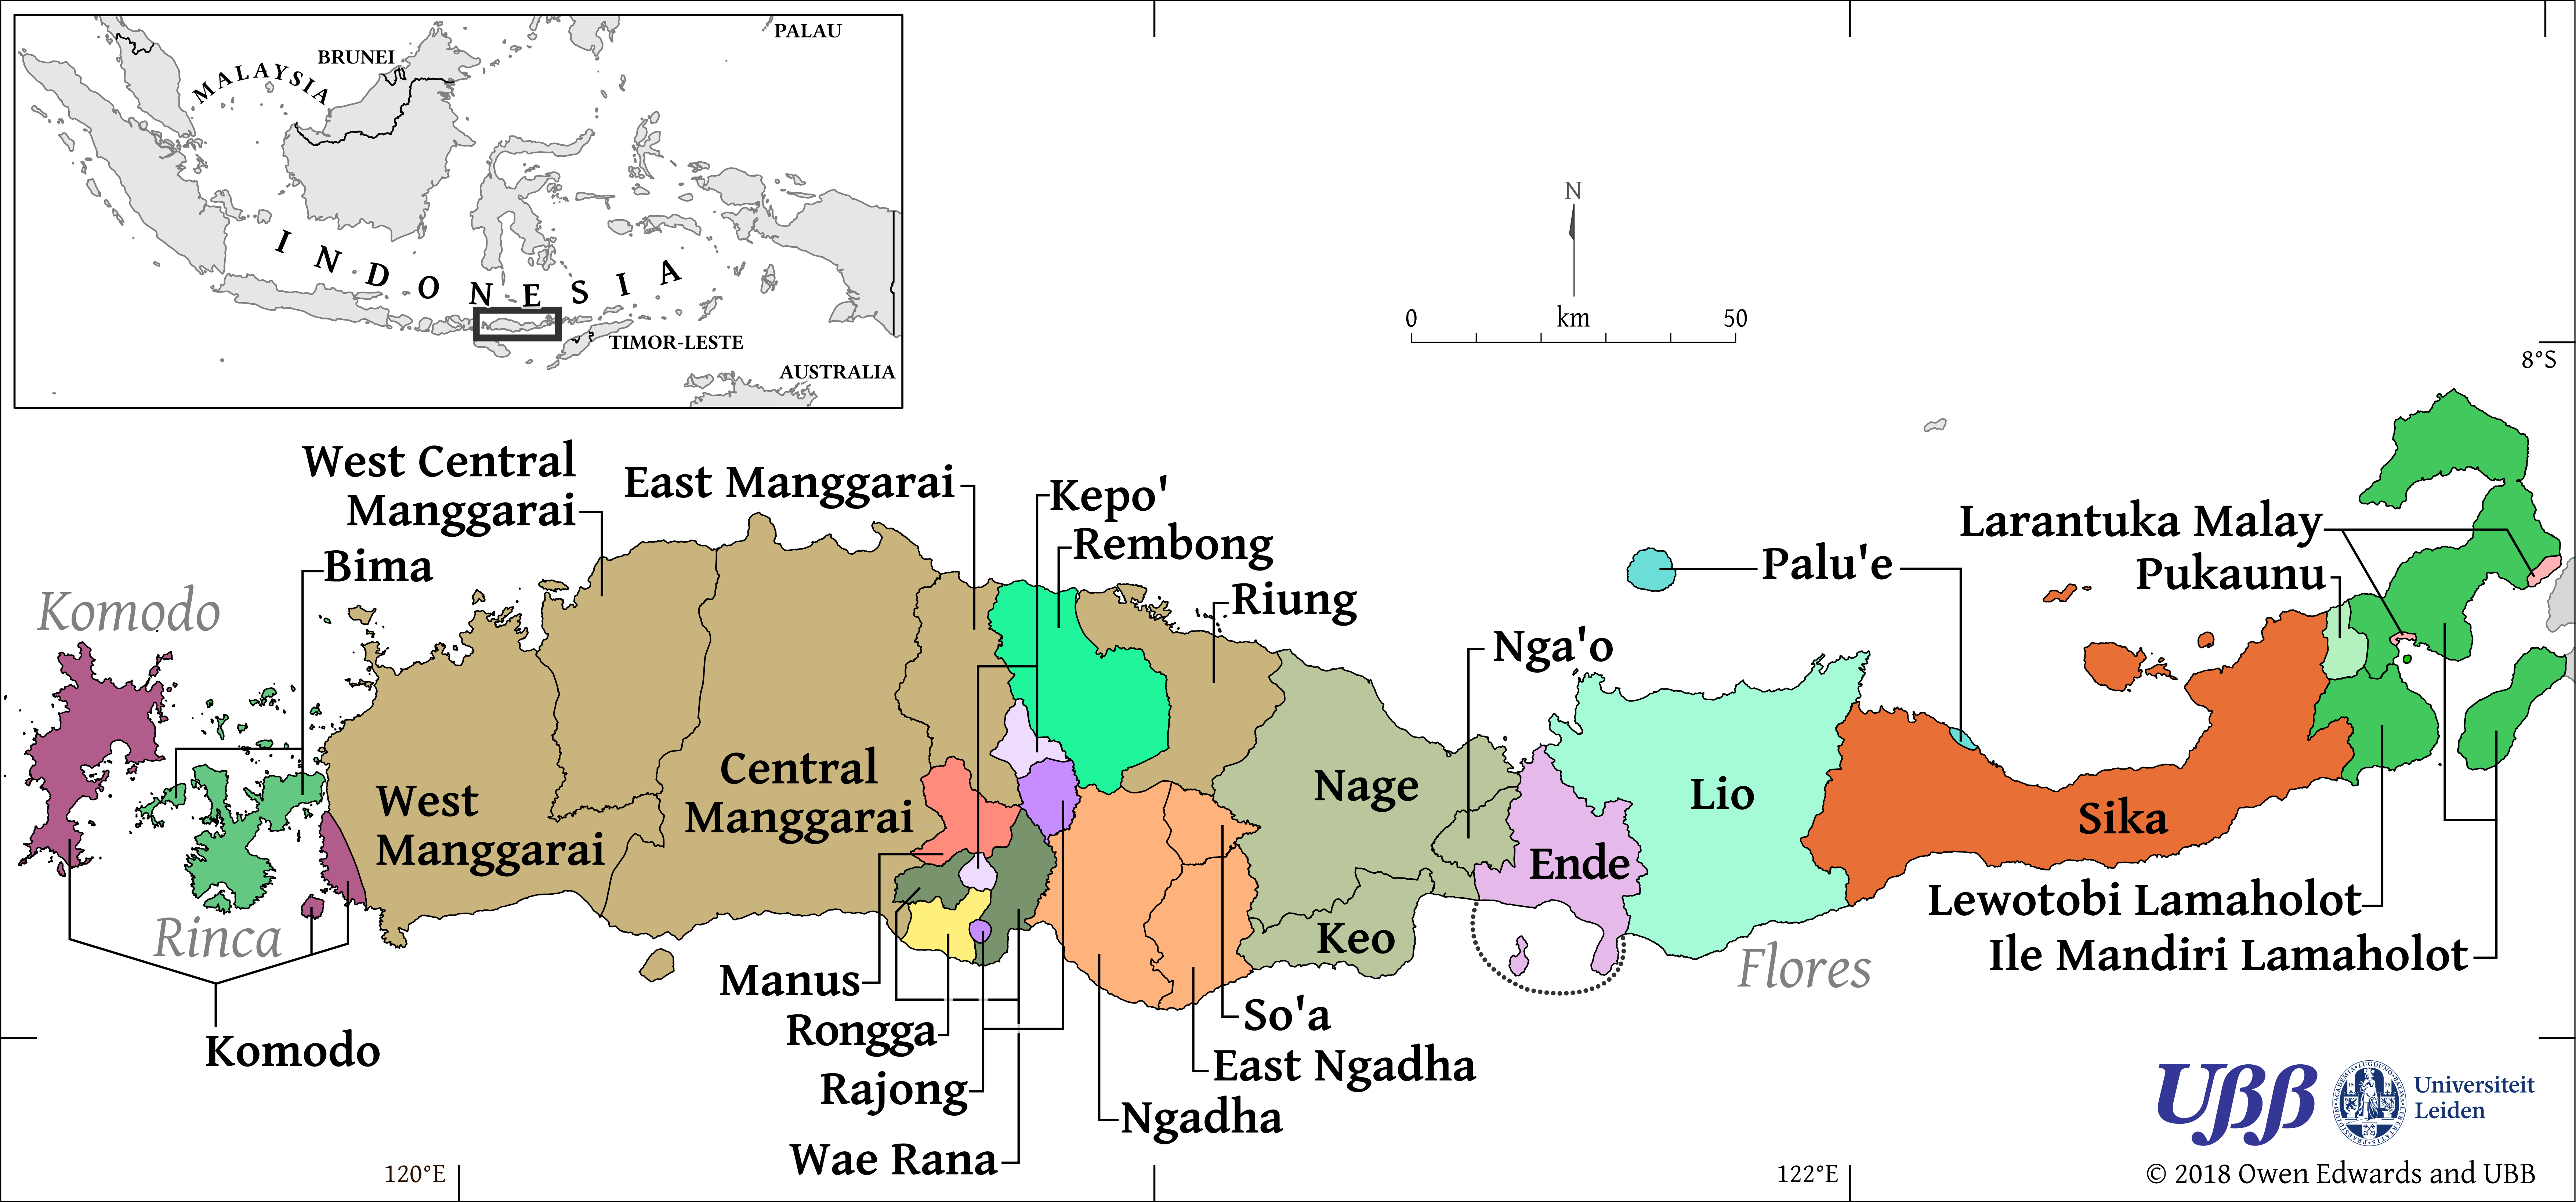
\includegraphics[width=0.9\linewidth] {Images/flores_languages__inset_.png}

\caption{Language map of the island of Flores \citep{edwards_ubb_2018}}
\label{fig:langmap}
%where in the world is the region in the map? Need one with a larger scope
\end{figure}

A few documents exist on Hewa. There is one wordlist by Marian Klamer \citep{klamer_2015}, as well as a few materials from Hanna Fricke, among them a sketch grammar \citep{Fricke2014} and a dictionary \citep{fricke_2015}. 

%Consultant and fieldwork

The present documentation project has taken place during a course in Field Methods as part of the MA Linguistics programme at Leiden University in the fall of 2021. Our language consultant is Eman, a 30 year-old student. He speaks Hewa natively and he is also fluent in Indonesian and English. He has spent a large part of his youth away from home, in different parts of Indonesia as well as in the Netherlands, meaning that he has had considerable contact with other languages, but he continues to use Hewa to communicate with his family. 

The present project has a few main outputs: on one hand, the documentation output, with recordings consisting of audio (WAV) and video (mp4) files recorded with a hand-held camera with an external microphone, an audio recorder, and mobile phones. These were made in the classroom during teaching hours as well as during private meetings with the consultant.

On the other hand, the description of the language consists of this sketch grammar, as well as a glossed text (see appendix \ref{sec:text})  and a list (see appendix \ref{sec:wordlist}) of all the vocabulary compiled during the project.

\end{document}